%
% sec-3-design.tex
%
% Embedded languages, stratified types, richly typed terms, representing
% programs. The Accelerate language.
%
% Accelerate CUDA backend. Code generation. Executing computations. Garbage
% collection. Caching.
%

% Need a better title
\chapter{Basics}  % Design of an embedded language
\epigraph{You see a wile, you thwart. Am I right?}%
{\textsc{---terry pratchett and neil gaiman}\\\textit{Good Omens}}


\section{Data Parallelism}
\label{sec:data_parallelism}

The major processor manufacturers and architectures have long since run out of
room with most of the traditional approaches to boosting CPU performance.
Instead of driving clock speed and straight-line instruction throughput,
including multiple cores on a single chip has become the dominant mechanism for
scaling processor performance. Despite this trend being apparent for a number of
years, programming parallel computers remains an extremely challenging task ---
even for expert computer programmers, let alone for scientists in other
disciplines.

One programming model that has shown to make good use of parallel hardware is
\indexe{data parallelism}.
% The idea is that the application of an operation over
% a collection of data, such as an array, can often be performed in parallel.
Data parallelism focuses on distributing the data over the available processors,
and for each processor to perform the \emph{same} task on the \emph{different}
pieces of distributed data. To the programmer, data parallelism exposes a single
logical thread of execution that is fairly easy to understand and reason about.
In addition to its simplicity, the data parallel approach to programming
parallel computers has several advantages:
%
\begin{enumerate}
\item The model is independent of the number of processors, so scales to any
    number of processors by decomposing data into the appropriate number of
    chunks.

\item All synchronisation is implicit, so the programming model is safe from
    race conditions, eliminating a major source of errors in parallel programs.

\item As memory bandwidth is often a limiting factor in modern computers, the
    emphasis on data layout can assist with both data flow as well as
    parallelisation.
\end{enumerate}
%
In the world of massively parallel computing with strong locality requirements,
data parallelism is the well established, demonstrably successful brand leader.
Examples of data parallel programming environments include High Performance
Fortran (HPF)~\cite{HPF:1997}, the collective operations of the Message Passing
Interface (MPI)~\cite{MPI:2012}, Google's Map/Reduce
framework~\cite{Dean:2008fi}, and NVIDIA's CUDA API for graphics
processors~\cite{NVIDIA:2012wf}.


\section{GPU computing} % {GPGPU programming is data parallel programming}
\label{sec:gpu_computing}

General-purpose computing on graphics processing units
(\indext{GPGPU}\index{GPGPU|see {general-purpose computing on graphics
processing units}}) is the utilisation of a graphics processing unit (\GPU),
which typically handles the computations for computer graphics, to perform
computations in applications typically handled by the central processing unit
(CPU). Since general purpose CPUs are designed to optimise the performance of a
single thread of execution, much of the processor's resources (die area and
power) to non-computational tasks such as caching and branch prediction.
Conversely, the highly parallel nature of graphics processing (rasterisation)
means the GPU architecture instead uses these resources to be able to execute
many tasks in parallel, improving the computational throughput for parallel
workloads at the expense of decreased single threaded performance. This
difference in architectures between the CPU and GPU is illustrated in
Figure~\ref{fig:cpu_gpu_block_diagram}.

\begin{figure}[tbp]
    \centering
    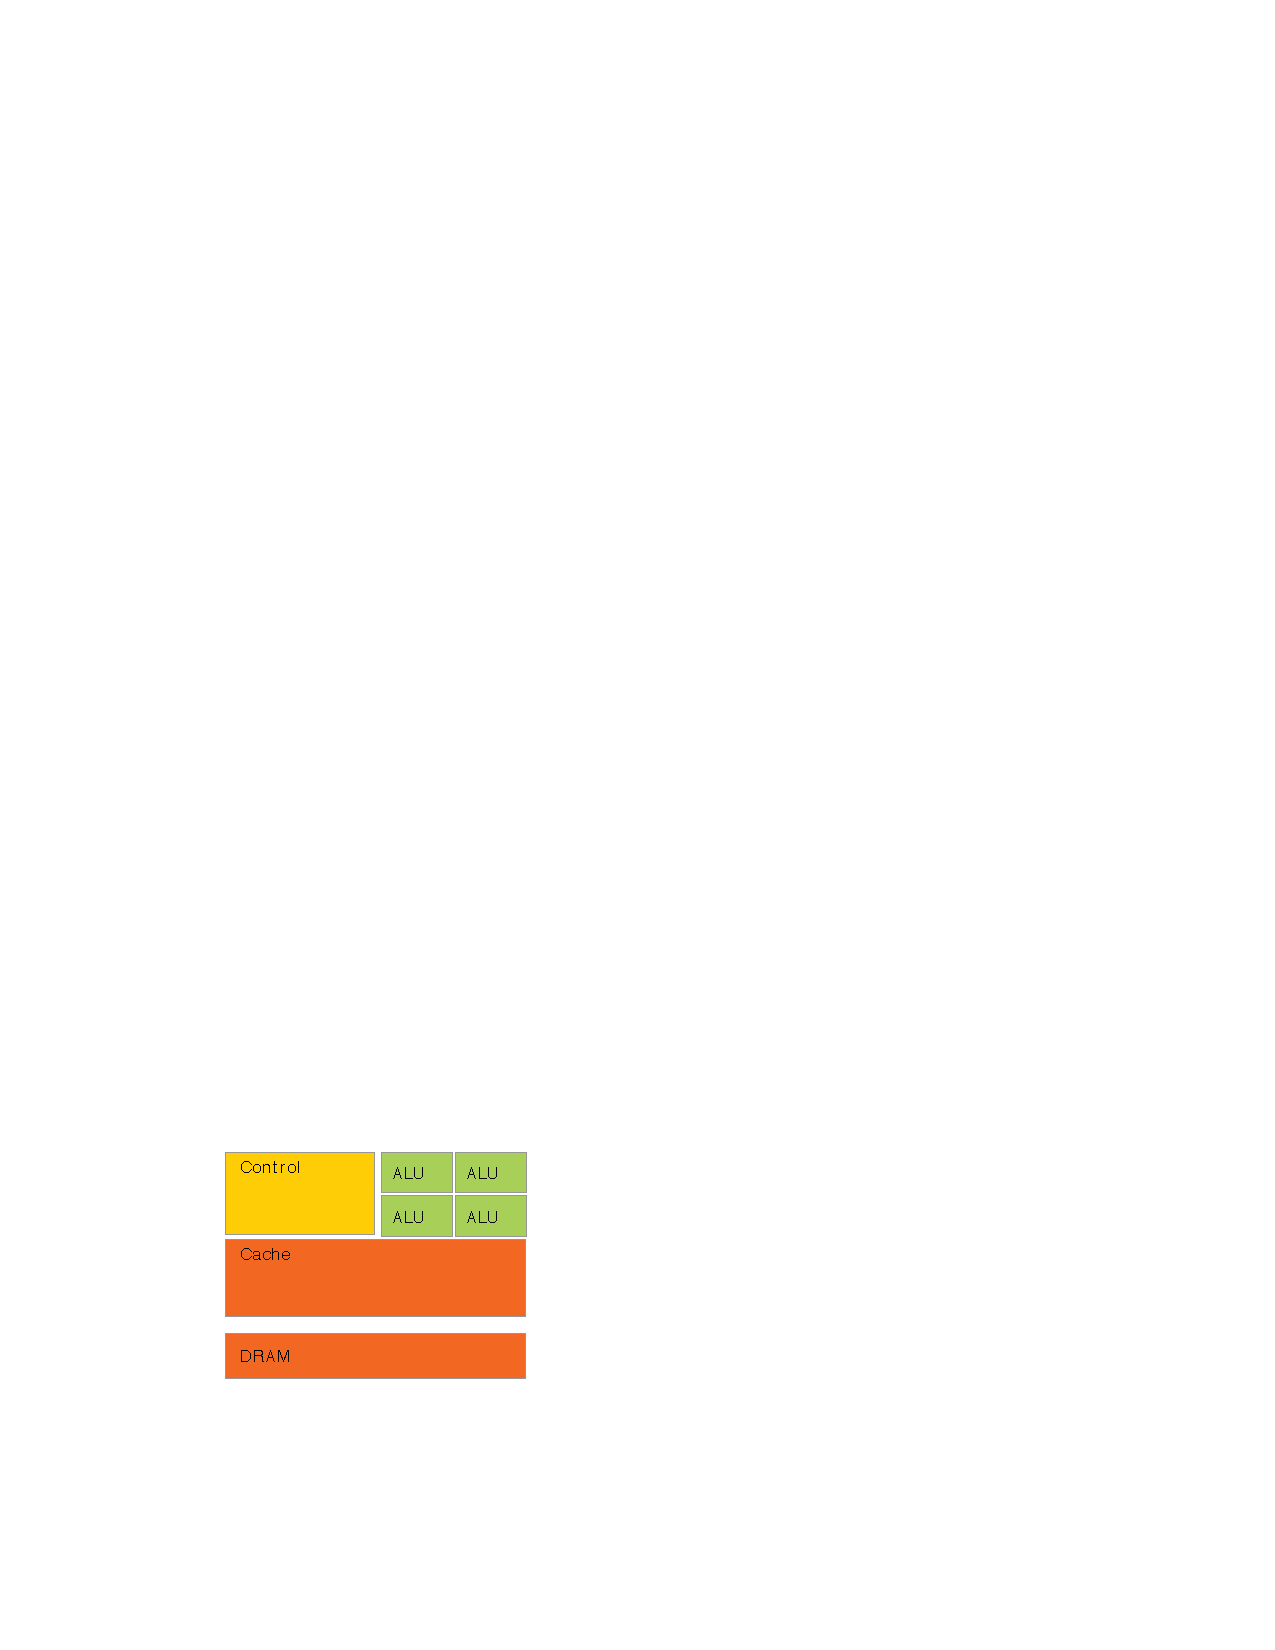
\includegraphics[width=0.4\textwidth]{images/sec-3/block_cpu}
    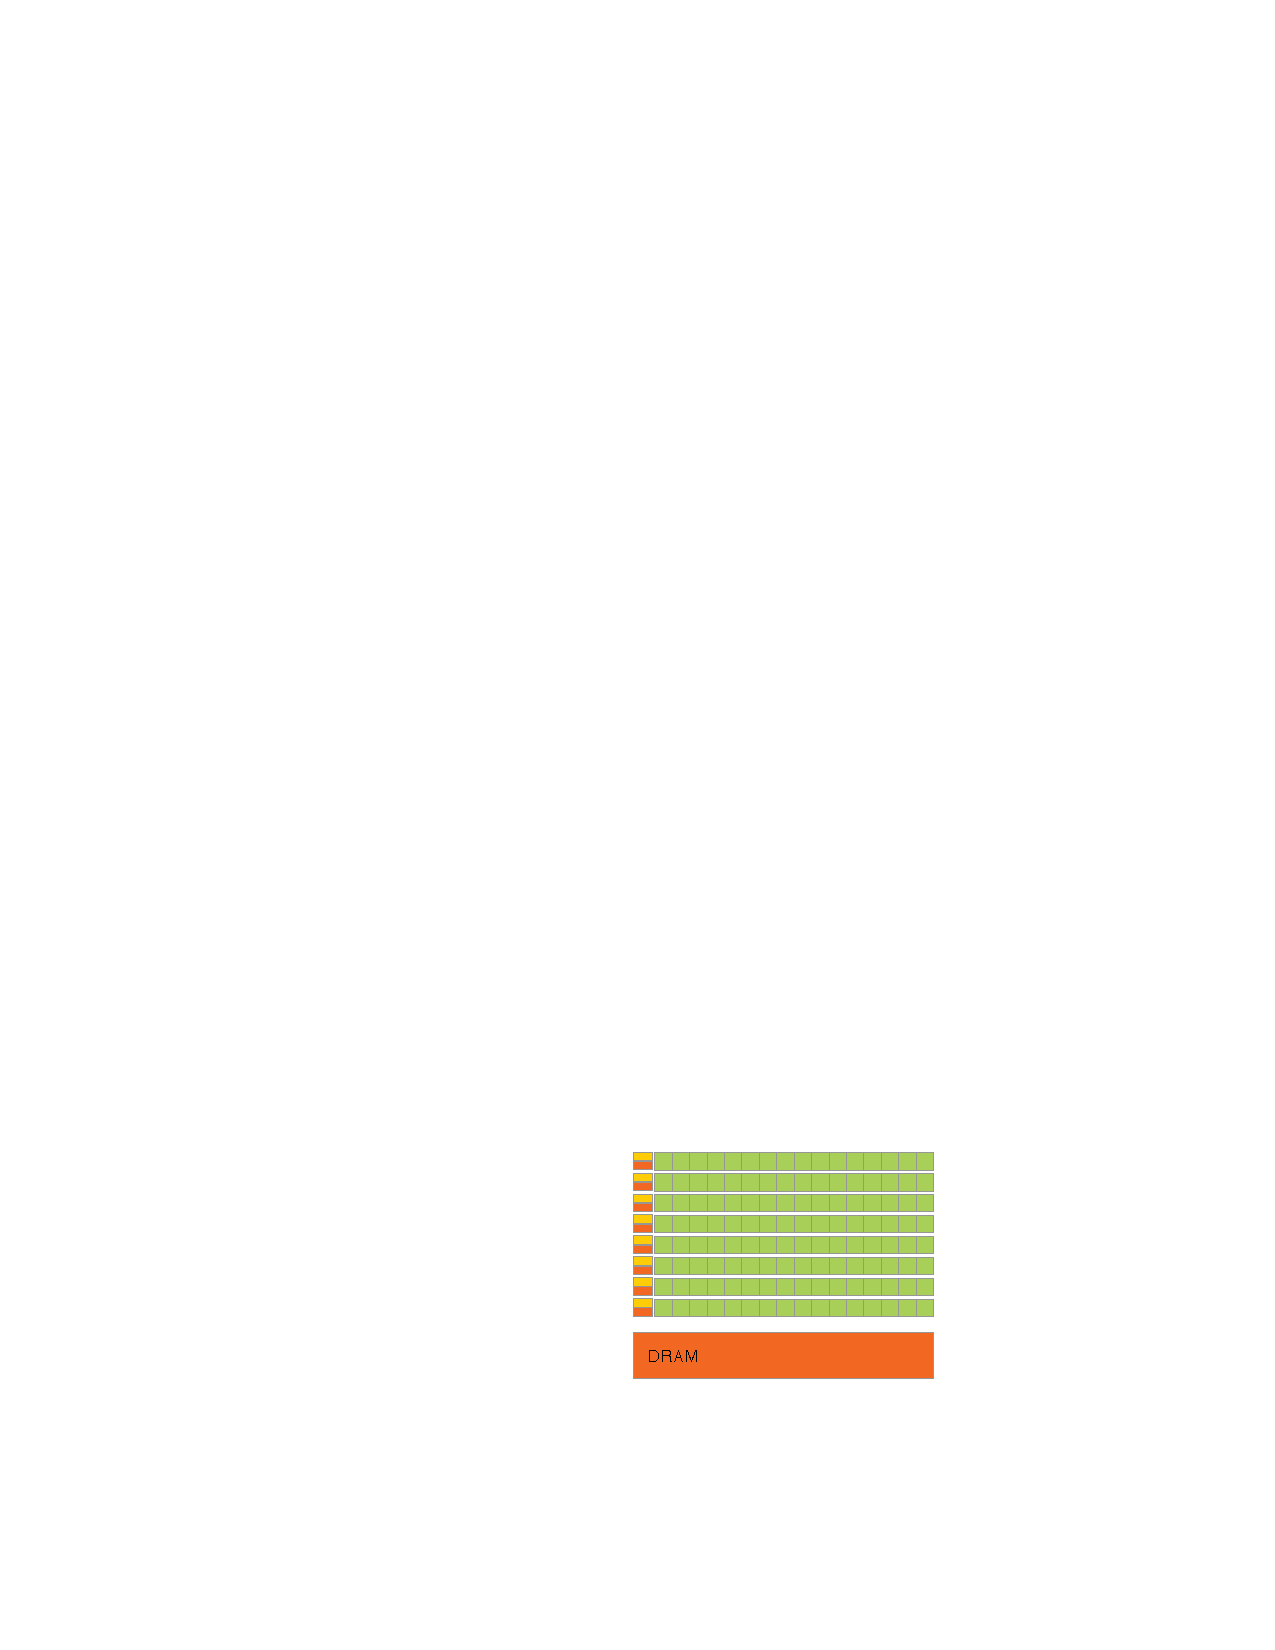
\includegraphics[width=0.4\textwidth]{images/sec-3/block_gpu}
    \caption[The GPU devotes more transistors to data processing]{Block diagram
    comparing the relative use of transistors in a CPU (left) compared to a GPU
    (right). The GPU is specialised for highly parallel, compute intensive
    workloads, and so is designed such that the majority of its transistors are
    devoted to data processing, rather than data caching and control flow.
    Images from~\cite{NVIDIA:2012wf}.}
    \label{fig:cpu_gpu_block_diagram}
\end{figure}

More specifically, the GPU is especially well suited to expressing problems that
can be expressed as data parallel computations, where the same program is
executed by many processors on many different data elements in parallel
(\S\ref{sec:data_parallelism}). Because the same program is executed by many
processors, there is no need for sophisticated control flow, and because it is
executed on many data elements, memory access latency can be hidden with
calculations rather than by big caches. Many applications that process large
data sets can use the data parallel programming model to speed up calculations,
and these applications can be coded to execute on the GPU.


\subsection{CUDA}
\label{sec:cuda}

\CUDA is the parallel computing platform and programming model created by
NVIDIA, which gives programmers direct access to the memory and parallel
computation units of their GPUs. Using CUDA, the massively parallel multicore
architecture of the GPU becomes accessible for general purpose computing, not
just graphics.

CUDA extends the C programming language by allowing the C programmer to define
functions, called \emph{kernels}\index{GPU!kernel}, that, when called, are
executed $n$ times in $n$ data parallel threads on the available processing
elements, rather than only once like regular C functions. These functions are
executed by threads arranged in a multidimensional structure of \emph{thread
blocks}\index{GPU!thread block}. Threads within a block can cooperate by sharing
data through some \emph{shared memory}\index{GPU!shared memory} and by
synchronising their execution to coordinate memory access. More precisely, the
programmer can specify synchronisation points in the kernel by calling
@__syncthreads()@\index{GPU!\code{__syncthreads()}}, which acts as a barrier at
which all threads in the block must wait before any is allowed to proceed. Each
thread block executes independently of each other, so a GPU with a higher number
of CUDA cores --- or \emph{streaming multiprocessors}\index{GPU!streaming
multiprocessor} (SM) --- will execute the program in less time than a GPU with
fewer multiprocessors.

\begin{lstlisting}[style=cuda
    ,float
    ,label=lst:cuda_vecadd
    ,caption={[CUDA kernel for pair wise addition of two vectors]A CUDA kernel
        that illustrates pair wise addition of two vectors. The
        \code{__global__} keyword marks a function as a kernel that should be
        executed on the GPU in data parallel. The execution configuration syntax
        \code{<<<...>>>} specifies the number of threads that will each execute
        the function in data parallel.}]
// Kernel definition
__global__ void VecAdd(float *A, float *B, float *C, int N)
{
    int i = blockIdx.x * blockDim.x + threadIdx.x;

    if (i < N) {
        C[i]  = A[i] + B[i];
    }
}

int main()
{
    ...
    // Kernel invocation with N threads
    int threadsPerBlock = 128;
    int numBlocks       = (N + threadsPerBlock - 1) / threadsPerBlock;
    VecAdd<<<numBlocks, threadsPerBlock>>>(A, B, C, N);
    ...
}
\end{lstlisting}

At an example, Listing~\ref{lst:cuda_vecadd} illustrates the pair wise addition
of two vectors $A$ and $B$ of size $N$ each, and stores the result in a vector
$C$. The kernel is defined with the @__global__@ declaration specifier. The
number of CUDA thread blocks and the number of threads in each block that
execute the kernel, at this invocation, is specified in the @<<<...>>>@ syntax.
Moreover, Listing~\ref{lst:cuda_vecadd} demonstrates that the GPU programming
model as exposed by CUDA is a data parallel programming model --- $N$ threads
execute $N$ individual instances of the kernel function @VecAdd@, and each
thread operates on a single element of each input array to create a single value
in the result.


\section{Embedded domain-specific languages}
\label{sec:EDSLs}

A \indexe{domain-specific language} (DSL) is a computer language specialised to
a specific problem domain. The DOT language~\cite{Graphviz:1998ui,Ellson:2001wf}
is an example of a DSL for describing graphs. This is in contrast to a general
purpose language such as Haskell~\cite{Haskell:1998}, which is broadly
applicable across domains but may lack specialised features for a particular
domain. A domain specific language is created to solve problems in a particular
domain, and is not intended to solve problems outside it (although this may be
technically possible). Restricting the problem domain the language is intended
to solve may allow for more optimisations during compilation, or increased
expressivity when representing problems or defining solutions in that domain.

An \emph{embedded} (or \emph{internal}) \emph{domain-specific
language}\index{domain-specific language!embedded} (EDSL) is a domain-specific
language that is designed to be used from within another host
language~\cite{Hudak:1996}. The embedded language is implemented as a library,
so is able to reuse the syntax and features of the general purpose host language
compiler, including compilation phases such as lexing, parsing, and semantic
analyses such as type checking, while adding domain specific elements such as
data types, or domain specific optimisations and code generation.

There are two major degrees in which an embedded language can be implemented:

\subsection{Shallow embedding}

In a shallow embedding, operations in the embedded language translate directly
into operations in the target language. A shallow embedding captures the
semantics of the data of the domain in a data type, and provides a \emph{fixed}
interpretation of that data. Thus, it is easy to add new constructs to the
language --- so long as they can be interpreted in the semantic domain --- and
the embedded language can reuse features of the host language, such as variable
binding.


\subsection{Deep embedding}

A deep embedding captures the semantics of the embedding by reflecting the
operations of the object language into a data structure. This data structure ---
an \indexe{abstract syntax tree} (AST) --- then permits transformations, such as
optimisations, before being translated into the target language. Deeply embedded
languages therefore enable a \emph{variable} interpretation of operations in the
domain, so it is easy to add new interpretations of the embedding, for example,
compiling to a different target language. However, adding new language
constructs requires extending the AST data type, and the implementation must
deal explicitly with binding of variables. Sharing and recursion are common
problems when implementing deeply embedded languages.

As the deeply embedded language runs inside of the host language, reflecting
operations into an AST, an interpreter for the embedded language must be
embedded within the host application.
% This interpreter may execute instructions in the internal language directly,
% or it may generate code that is compiled into machine language instructions to
% be executed.
As the interpreter executes code for the embedded language at program runtime,
code in the embedded language may either be written by the user or generated
dynamically by the application. If the target language is different to that of
the host language, this entails the interpreter generating, compiling, and
executing code for the target language at program runtime.


\section{The Accelerate EDSL}

The current generation of graphical processing units (GPUs) are massively
multicore processors (\S\ref{sec:gpu_computing}). They are optimised for
workloads with a large degree of data parallelism (\S\ref{sec:data_parallelism})
and good performance depends on highly idiomatic programs with low SIMD
divergence and regular memory-access patterns. Hence, the development of
applications that use the graphics processors for general purpose computations
(\S\ref{sec:gpu_computing}) is work intensive and requires a substantial degree
of expert knowledge.

Accelerate is our approach to reducing the complexity of GPU programming: a
high-level, deeply embedded domain-specific language (\S\ref{sec:EDSLs}) of
array computations that captures appropriate GPGPU idioms in the form of
parameterised, \emph{rank-polymorphic}~\cite{Keller:2010er}, collective
operations on arrays~\cite{Chakravarty:2011fr}. Our choice of operations was
informed by the \emph{scan-vector model}~\cite{Chatterjee:1990vj}, which is
suitable for a wide range of algorithms, and demonstrated that these operations
can be efficiently implemented on modern GPUs~\cite{Sengupta:2007tc}.

We regard Accelerate's collective array operations as algorithmic
skeletons~(\S\ref{sec:code_generation}) that capture appropriate GPU programming
idioms. The dynamic code generator instantiates CUDA implementations of these
skeletons~(\S\ref{sec:parallel_algorithms_in_cuda}) to implement embedded array
programs~(\S\ref{sec:instantiating_skeletons}). Dynamic code generation exploits
runtime information of the target hardware to optimise GPU code, and enables
on-the-fly generation of embedded array programs by the host
program~(\S\ref{sec:dynamic_compilation}). The evaluator minimises the overhead
of dynamic code generation by caching binaries of previously compiled skeleton
instantiations and by parallelising code generation, data
transfer~(\S\ref{sec:memory_management}), and GPU kernel loading, configuration,
and execution~(\S\ref{sec:executing_programs}).

The achieve performance competitive with hand-written
CUDA~\cite{McDonell:2013wi}, we implement two primary optimisation techniques:
sharing recovery~(\S\ref{sec:sharing_recovery}) tackles code explosion due to
the embedding in Haskell, while array
fusion~(\S\ref{sec:implementing_array_fusion}) eliminates superfluous
intermediate structures, which often arise due to the high-level nature of the
language. Both of these techniques are well known from other contexts, but they
present unique challenges for an embedded language compiled for execution on a
GPU.



\endinput

MMTC: Chapter 2 (Background): Don't bother introducing Haskell and things like
parallelism vs concurrency etc. What you need to discuss is (1) data parallelism
and (2) how GPGPU programming is data parallel programming. Then, (3) the idea
of embedded languages and runtime code generation. However, don't go into too
much details at this point. After all, much of this has been discussed in
existing literature already. I'd suggest to pick 1-2 examples and use them to
drive the explanations (and at the same time give people an idea for the feel of
Accelerate programs).


MMTC: Chapter 3 (Design): Maybe you should call the chapter ``Design and Related
Work''. It seems that you want to cover related work there and it is a good idea
to make that easy to find.

MMTC: More generally, there are two ways to do related work. Everything in one
related work chapter or have a related work section at the end of each chapter.
The latter works better if there is different sorts of related work for the
different chapters. This may apply here as, eg, the related work for embedded
languages and the related work for fusion has little overlap. (You can look at
my thesis for an example of that style.)


\begin{itemize}
\item Why another parallel programming language? (1 day)

\item Accelerate design (3 weeks)
    \begin{itemize}
        \item rank-polymorphic array language of collective operations
        \item programming model
        \item algorithmic skeletons
        \item stratified language: using the type system to exclude nesting
        \item richly typed terms; environments \& types (type safe evaluator)
        \item types help catch bugs in the compiler; important since
            compilation happens at program \emph{runtime}
        \item surface vs.\ internal (core) languages
            %\item representing different constructs (c.f. nesting?)
        \item examples: operator expressiveness (application driven)
    \end{itemize}

\end{itemize}


